\documentclass{ximera}

\begin{document}

    \title{Lecture 3}
    
    \begin{abstract} 
    - IEEE standard: double precision \\
    - Big O, little O notation \\
    - BLAS and LAPACK introduction
    \end{abstract}
    \maketitle

REVIEW

Precision 

\textit{Relative Representation Error}
    The expression $.31416\times 10^1$ has five significant figures, and thus if this is the highest precision representation of a number on a computer, any information less than $.5\times 10^4$ is lost.  Thus, the \textcolor{red}{relative representation error} is
    \begin{align}
        \frac{|x-.31416\times 10^1|}{.31416\times 10^1} \leq \frac{.5\times 10^4}{.31416\times 10^1} \approx .16 \times 10^4
    \end{align}
    The maximum relative representation error in a normalized number occurs for $.10000\times 10^1$, which is the most accurate five-digit approximation of all numbers in $[.999995, 1.00005]$.  The relative error is therefore bounded by $.5\times 10^{-4}$.  
    \begin{definition}
        The maximum relative representation error in a floating point arithmetic with $p$ digits and base $\beta$ is $.5\times \beta^{1-p}$. (Note that this is half the distance between 1 and the next largest floating point number, $1+\beta^{1-p}$.)
    \end{definition}

\textit{Single Precision}
\begin{itemize}
    \item If the sign $s$, exponent $e$, and fraction $f<1$ are 1-bit sign, 8-bit exponent, and 23-bit fraction in IEEE triple precision format, respectively, then the number is represented by $(-1)^s \cdot 2^{e-127}\cdot(1+f)$
    \item Maximum relative representation error: $2^{-24} \approx 6\times 10^{-8} = \mathcal{O}(10^{-7})$
    \item Range of positive normalized numbers: $[2^{-126}, 2^{127}]$ ([underflow threshold, overflow threshold])
\end{itemize}

WHERE WE LEFT OFF

\begin{center}
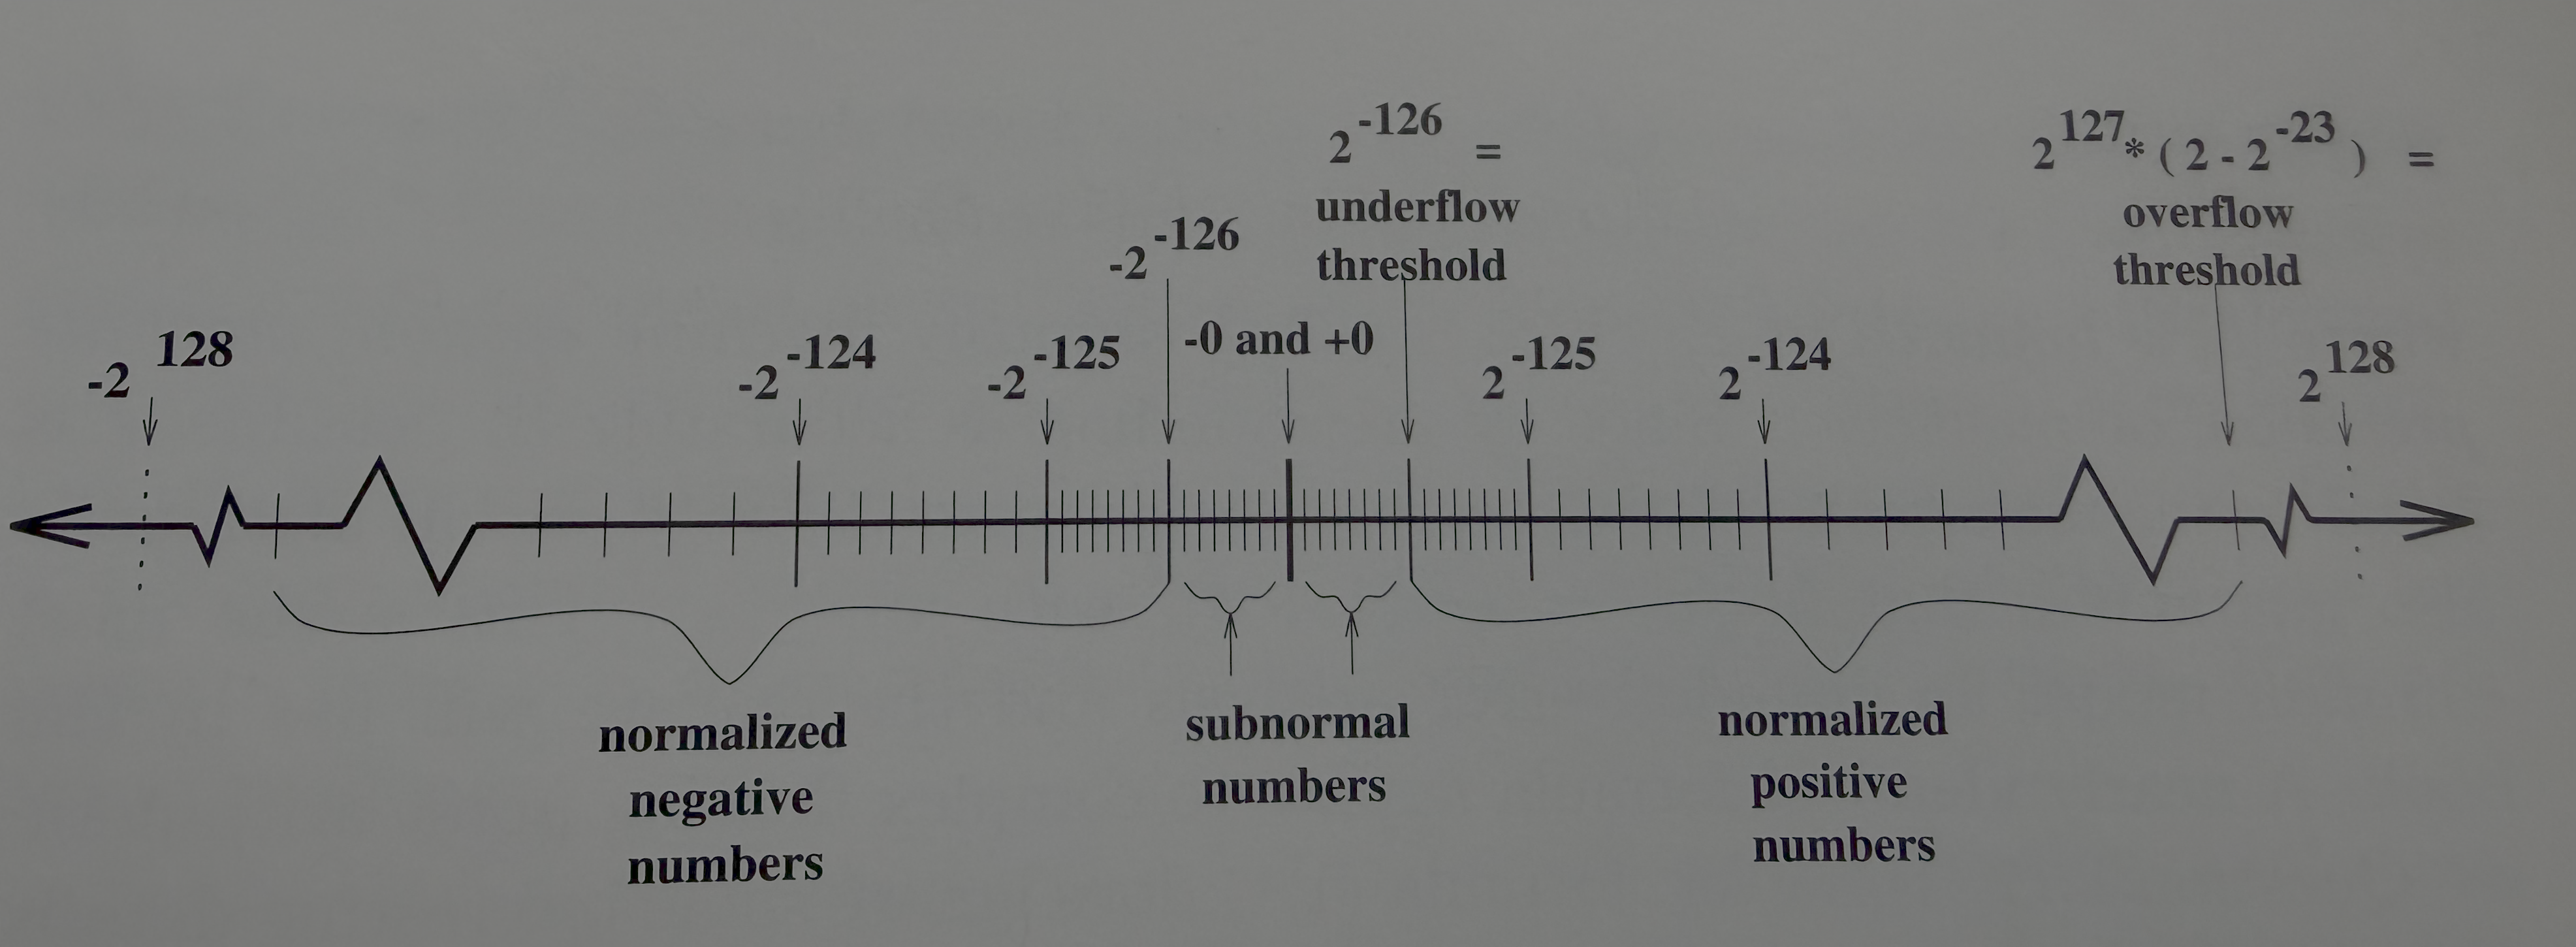
\includegraphics[width=0.85\textwidth]{xmPictures/ieee_scale_singlePrecision.png}
\end{center}

\textit{Double Precision}
\begin{itemize}
    \item If the sign $s$, exponent $e$, and fraction $f<1$ are 1-bit sign, 11-bit exponent, and 52-bit fraction in IEEE triple precision format, respectively, then the number is represented by $(-1)^s \cdot 2^{e-1023}\cdot(1+f)$
    \item Maximum relative representation error: $2^{-24}\approx 10^{-16}$
    \item Range of positive normalized numbers: $[2^{-1022}, 2^{1023}\cdot (2-2^{-52})\approx 2^{1024}]$ ([underflow threshold, overflow threshold])
\end{itemize}

\textit{IEEE Arithmetic}
\begin{itemize}
    \item If a flop $\odot$ does not produce an exact floating point number, i.e. $a\odot b \neq \text{fl}(a\odot b)$, where $\text{fl}(a\odot b)$ is the nearest floating point number to $a \odot b$, there is \textcolor{red}{roundoff error} equal to $a\odot b - \text{fl}(a\odot b)$.
    \item Can write $\text{fl}(a\odot b) = (a \odot b)(1+\delta)$ where $|\delta|$ is bounded by $\epsilon$ called \textcolor{red}{machine epsilon, machine precision, or macheps}, equal of course to the maximum relative representation error
    \item IEEE arithmetic also guarantees that $\text{fl}(\sqrt(a)) = \sqrt{a}(1+\delta)$
    \item IEEE arithmetic is designed to preserve as many mathematical relationships as possible
\end{itemize}

Now a brief aside:  when determining how expensive an algorithm is, we are adding up the number of flops we are doing.  For example, one multiplication is 1 flop, while the multiplication of two $n \times n $ matrices is $n^3$ flops. If we multiply  two $n\times n$ matrices, and then add ones along the diagonal of the resulting product, that is $n^3 + n$ flops.  As $n$ gets large, we only care about the largest value in terms of compute time.  The notation $\mathcal{O}$ is used to identify this largest degree term in the polynomial, so $n^3 + n$ would be called an $\mathcal{O}(n^3)$ algorithm.  There are more precise definitions, and even a little ``o" notation $\mathcal{o}$, but we won't be needing much of that in this course.  Storage, i.e. assigning a spot in memory for a vector or a matrix, costs the same number of flops as there are entries in the object: e.g., it costs $m\times n$ flops to store a $m\times n$ matrix.

Designing algorithms to minimize precision error is a fundamental aspect of designing numerical algorithms.  The package BLAS, abbreviation for Basic Linear Algebra Subprograms, and LAPACK, short for Linear Algebra Package.  Nearly all programming languages use these packages, each of which have built in optimal methods for solving linear algebra problems under the constraints of IEEE arithmetic.  
\begin{itemize}
    \item Level $1$ BLAS includes operations that are $\mathcal{O}(n)$, such as vector addition, dot products, and plane rotation
    \item Level 2 BLAS includes operations that are order $\mathcal{O}(n^2)$, such as matrix-vector multiplication and order $\mathcal{O}(n^2)$ updates to matrices
    \item Level 3 BLAS includes operations that are order $\mathcal{O}(n^3)$ operations such as matrix-matrix multiplication and triangular solve
\end{itemize}

\textbf{Throughout this course, we will investigate not only different ways of using linear algebra to identify different properties of the image space, but also explain when the numerics requires new innovation and techniques to implement what are theoretically intuitive algorithms. One of our first examples will be Gram-Schmidt orthogonalization.}

\end{document}



